%!TEX root = ../my_thesis.tex
\section[Physics of the neutral $B$ mesons]{Physics of the neutral \boldmath{$B$} mesons}
\label{sec:Bphysics}

The theory of neutral $B$ meson oscillation, decays and \CP~violation presented here is derived from Refs.~\cite{PDG,CPviolation}.

\subsection{Oscillation of neutral mesons}

Neutral $B$ meson states are characterised by the following quark content:
\begin{align}
	\ket{B^0} &= \ket{d\bar b}, & \ket{\bar B^0} &= \ket{\bar d b}, \\
	\ket{B_s^0} &= \ket{s\bar b}, & \ket{\bar B_s^0} &= \ket{\bar s b}. 
\end{align}
All neutral mesons will be denoted as $P^0$ or $\bar P^0$ hereafter. The $\bar P^0$ state is obtained from $P^0$
via the \CP~operator up to an arbitrary phase factor $e^{i\phi_{CP}}$.
Since charged currents do not conserve flavour quantum numbers (e.g. strangeness, beauty etc\dots),
a neutral meson can transform itself into its own anti-meson, and vice versa. 
So, the time evolution of a neutral $B$ meson system can be generally written as
\begin{equation}
	\ket{\Psi(t)} = a(t)\ket{P^0} + b(t)\ket{\bar P^0} + \sum_i c_i(t) \ket{f_i},
\end{equation}
where $\ket{f_i}$ are all the possible final states with $c_i(0)=0$ as initial condition.

Since the typical timescale of weak interactions is much longer than the strong interaction timescale,
we can neglect all weak interactions among final states (\emph{Weisskopf-Wigner approximation}). 
So, we can write the Schroedinger equation for $\ket{\Psi(t)}$ in terms of an effective, non-hermitian 
hamiltonian $\mathcal H$:
\begin{equation}
	\label{eq:schroedinger}
	i\partial_t \left( \begin{array}{c} a(t) \\ b(t) \end{array} \right) = \mathcal H \left( \begin{array}{c} a(t) \\ b(t) \end{array} \right) = 
	\left( \begin{array}{cc} H_{11} & H_{12} \\ H_{21} & H_{22} \end{array} \right) \left( \begin{array}{c} a(t) \\ b(t) \end{array} \right). 
\end{equation} 
The $\mathcal H$ matrix can be rewritten as the sum of two hermitian matrices $M$ and $\Gamma$:
\begin{equation}
	\label{eq:effhamiltonian}
	\mathcal H = M - \frac{i}{2} \Gamma = 
	\left( \begin{array}{cc} M_{11} & M_{12} \\ M_{21} & M_{22} \end{array} \right) - \frac{i}{2} \left( \begin{array}{cc} \Gamma_{11} & \Gamma_{12} \\ \Gamma_{21} & \Gamma_{22} \end{array} \right).
\end{equation}
Assuming $CPT$~invariance ($H_{11}=H_{22}=H_0$, $M_{11}=M_{22}=M_0$, $\Gamma_{11}=\Gamma_{22}=\Gamma_0$), the eigenvalues of $\mathcal H$ are
\begin{align}
	\lambda_{L} &= m_{L} - \frac{i}{2}\Gamma_{L} = H_0 + \sqrt{H_{12}H_{21}} = H_0 + \sqrt{\left(M_{12}-\frac{i}{2}\Gamma_{12}\right)\left(M_{12}^*-\frac{i}{2}\Gamma_{12}^*\right)}, \\
	\lambda_{H} &= m_{H} - \frac{i}{2}\Gamma_{H} = H_0 - \sqrt{H_{12}H_{21}} = H_0 - \sqrt{\left(M_{12}-\frac{i}{2}\Gamma_{12}\right)\left(M_{12}^*-\frac{i}{2}\Gamma_{12}^*\right)},
\end{align}
where $L$ (``light'') and $H$ (``heavy'') refer to the value of the mass for each eigenstate.
The corresponding eigenvectors are
\begin{align}
	\label{eq:eigenvectors}
	\ket{P_L} &= p\ket{P^0} + q\ket{\bar P^0}, & \ket{P_H} &= p\ket{P^0} - q\ket{\bar P^0},	
\end{align}
where $p$ and $q$ satisfy $|p|^2+|q|^2 = 1$ and are given by
\begin{equation}
	\frac{q}{p} = \sqrt{ \frac{H_{21}}{H_{12}} } = 
			\sqrt{ \frac{M_{21}-\frac{i}{2}\Gamma_{21}}{M_{12}-\frac{i}{2}\Gamma_{12}} } =
			 \sqrt{ \frac{M^*_{12}-\frac{i}{2}\Gamma^*_{12}}{M^*_{21}-\frac{i}{2}\Gamma^*_{21}} }.  
\end{equation}
The relative phase $\phi_M$ between $M_{12}$ and $\Gamma_{12}$ is an observable quantity describing indirect \CP~violation (Sec.~\ref{sec:cpv}):
\begin{align}
	M_{12} &= M_{12}^*e^{i\phi_{CP}}, & \Gamma_{12} &= \Gamma_{12}^*e^{i\phi_{CP}}e^{i\phi_M}.
\end{align}
For the neutral $B$ meson system, the ratio $|\Gamma_{12}/M_{12}|$ is expected to be small in the SM; as a consequence, it can be shown that
\begin{equation}
	\label{eq:pqratio}
	\frac{q}{p} = -e^{-i\phi_M} \left[1-\frac{1}{2}\left|\frac{\Gamma_{12}}{M_{12}}\right|\sin\phi_M + \mathcal O\left( \left|\frac{\Gamma_{12}}{M_{12}}\right|^2 \right) \right],
\end{equation}
which implies $|q/p|\sim1$.

The difference and the average of the masses and widths of the two mass eigenstates are defined as
\begin{align}
	\label{eq:deltaM}
	\Delta m &= m_H - m_L = \Re(\lambda_H - \lambda_L), & m &= \frac{m_L+m_H}{2} = \frac{\Re(\lambda_H + \lambda_L)}{2}, \\
	\label{eq:deltaGamma}
	\Delta\Gamma &= \Gamma_L - \Gamma_H = -2\Im(\lambda_L - \lambda_H), & \Gamma &= \frac{\Gamma_L+\Gamma_H}{2} = -\frac{\Re(\lambda_H + \lambda_L)}{4}. 
\end{align}
The sign convention for $\Delta\Gamma$ is chosen to have a positive experimental value for the $B^0_s$ system (for $B^0$, experiments give a result compatible with zero, in agreement with the SM).

The time evolution of the states $\ket{P^0(t)}$ and $\ket{\bar P^0(t)}$ when they are initially produced as $\ket{P^0(0)}$ and $\ket{\bar P^0(0)}$ can be obtained from the effective hamiltonian:
\begin{align}
	\ket{P^0(t)} &= g_+(t) \ket{P^0(t)} + \frac{q}{p} g_-(t) \ket{\bar P^0(t)}, \\
	\ket{\bar P^0(t)} &= g_+(t) \ket{\bar P^0(t)} + \frac{p}{q} g_-(t) \ket{P^0(t)}.
\end{align}
The functions $g_{\pm}(t)$ are built in terms of the eigenvalues:
\begin{equation}
	g_{\pm}(t) = \frac{1}{2} \left( e^{-im_H t-\frac{1}{2}\Gamma_H t} \pm e^{-im_L t-\frac{1}{2}\Gamma_L t} \right).
\end{equation}
The probabilities that a state initially produced as $P^0$ or $\bar P^0$  becomes a $P^0$ or $\bar P^0$ at~time~$t$~are
\begin{align}
	\left| \braket{P^0(0) | P^0(t) } \right|^2 &= |g_+(t)|^2 = \frac{e^{-\Gamma t}}{2} \left( \cosh\frac{\Delta\Gamma t}{2} + \cos\Delta m t \right), \\
	\label{eq:P0barToP0}
	\left| \braket{\bar P^0(0) | P^0(t) } \right|^2 &= \left| \frac{q}{p} \right|^2 |g_-(t)|^2 = \left| \frac{q}{p} \right|^2 \frac{e^{-\Gamma t}}{2} \left( \cosh\frac{\Delta\Gamma t}{2} - \cos\Delta m t \right), \\
	\label{eq:P0ToP0bar}
	\left| \braket{P^0(0) | \bar P^0(t) } \right|^2 &= \left| \frac{p}{q} \right|^2 |g_-(t)|^2 = \left| \frac{p}{q} \right|^2 \frac{e^{-\Gamma t}}{2} \left( \cosh\frac{\Delta\Gamma t}{2} - \cos\Delta m t \right), \\
	\left| \braket{\bar P^0(0) | \bar P^0(t) } \right|^2 &= |g_+(t)|^2 = \frac{e^{-\Gamma t}}{2} \left( \cosh\frac{\Delta\Gamma t}{2} + \cos\Delta m t \right).
\end{align}
The equations above describe the \emph{oscillation} of the $B^0$ and $B^0_s$ mesons.

\subsection{Decay of neutral mesons}
\label{sec:neutral_meson_decays}

The amplitude for the decay of a neutral meson into a final state $f$ can be obtained from the effective hamiltonian $\mathcal H$:
\begin{align}
	A_f &= \bra{f}\mathcal H \ket{P^0}, & \bar A_f &= \bra{f}\mathcal H \ket{\bar P^0}, \\
	A_{\bar f} &= \bra{\bar f}\mathcal H \ket{P^0}, & \bar A_{\bar f} &= \bra{\bar f}\mathcal H \ket{\bar P^0}.
\end{align}
After defining the parameters
\begin{align}
	\lambda_f &= \frac{q}{p}\frac{\bar A_f}{A_f}, & \frac{1}{\bar\lambda_{\bar f}} &= \lambda_{\bar f} = \frac{q}{p}\frac{\bar A_{\bar f}}{A_{\bar f}},
\end{align}
it is possible to write the \emph{decay rates} for neutral mesons decaying into $f$ or $\bar f$: 
\begin{equation}
	\label{eq:P0tof}
	\begin{split}
		\frac{d\Gamma(P^0\to f)}{dt}(t) &= N_f |A_f|^2 \frac{1+|\lambda_f|^2}{2}e^{-\Gamma t} \\
		& \left[ \cosh\left(\frac{\Delta\Gamma t}{2}\right) + D_f \sinh\left(\frac{\Delta\Gamma t}{2}\right) + C_f \cos \left( \Delta m t \right) - S_f \sin \left( \Delta m t \right) \right],   
	\end{split}
\end{equation}
\begin{equation}
	\label{eq:P0bartof}
	\begin{split}
		\frac{d\Gamma(\bar P^0\to f)}{dt}(t) &= N_f |A_f|^2 \left|\frac{p}{q}\right|^2 \frac{1+|\lambda_f|^2}{2}e^{-\Gamma t} \\
		& \left[ \cosh\left(\frac{\Delta\Gamma t}{2}\right) + D_f \sinh\left(\frac{\Delta\Gamma t}{2}\right) - C_f \cos \left( \Delta m t \right) + S_f \sin \left( \Delta m t \right) \right],   
	\end{split}
\end{equation}
\begin{equation}
	\label{eq:P0tofbar}
	\begin{split}
		\frac{d\Gamma(P^0\to \bar f)}{dt}(t) &= N_f |\bar A_{\bar f}|^2 \left|\frac{q}{p}\right|^2 \frac{1+|\bar \lambda_{\bar f}|^2}{2}e^{-\Gamma t} \\
		& \left[ \cosh\left(\frac{\Delta\Gamma t}{2}\right) + D_{\bar f} \sinh\left(\frac{\Delta\Gamma t}{2}\right) + C_{\bar f} \cos \left( \Delta m t \right) - S_{\bar f} \sin \left( \Delta m t \right) \right],   
	\end{split}
\end{equation}
\begin{equation}
	\label{eq:P0bartofbar}
	\begin{split}
		\frac{d\Gamma(\bar P^0\to \bar f)}{dt}(t) &= N_f |\bar A_{\bar f}|^2 \frac{1+|\bar \lambda_{\bar f}|^2}{2}e^{-\Gamma t} \\
		& \left[ \cosh\left(\frac{\Delta\Gamma t}{2}\right) + D_{\bar f} \sinh\left(\frac{\Delta\Gamma t}{2}\right) - C_{\bar f} \cos \left( \Delta m t \right) + S_{\bar f} \sin \left( \Delta m t \right) \right],
	\end{split}
\end{equation}
where $N_f$ is a time-independent normalisation factor and
\begin{align}
	\label{eq:cp_f}
	D_f &= -\frac{2\Re \lambda_f}{1+|\lambda_f|^2}, & C_f &= \frac{1-|\lambda_f|^2}{1+|\lambda_f|^2}, & S_f &= \frac{2\Im \lambda_f}{1+|\lambda_f|^2}, \\
	\label{eq:cp_fbar}	
	D_{\bar f} &= -\frac{2\Re \bar\lambda_{\bar f}}{1+|\bar\lambda_{\bar f}|^2}, & C_{\bar f} &= -\frac{1-|\bar\lambda_{\bar f}|^2}{1+|\bar\lambda_{\bar f}|^2}, & S_{\bar f} &= -\frac{2\Im \bar\lambda_{\bar f}}{1+|\bar\lambda_{\bar f}|^2}
\end{align}
are known as \emph{\CP~coefficients}.

\subsection[$CP$~violation in neutral meson systems]{\boldmath{$CP$}~violation in neutral meson systems}
\label{sec:cpv}

Three types of \CP~violation can occur. They are briefly sketched in Fig.~\ref{fig:CPVclasses} and described in the following paragraphs.

\begin{figure}[htbp]
  \begin{center}
    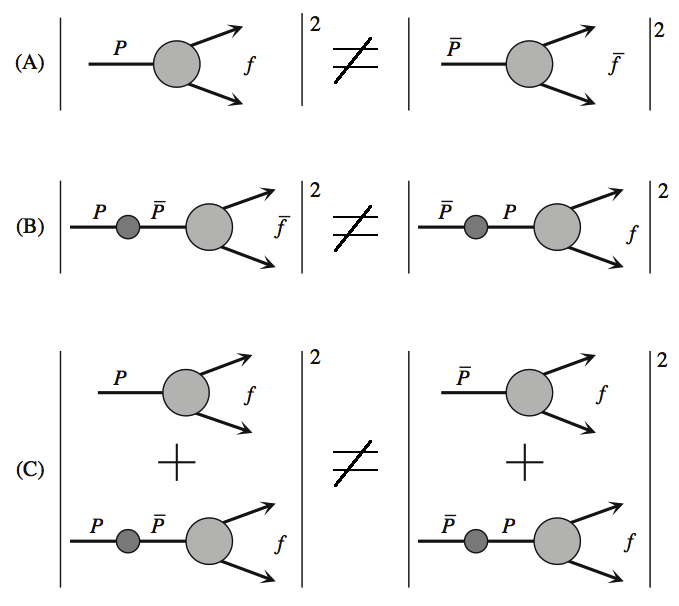
\includegraphics[width=0.9\textwidth]{03BPhysics/figs/CPVclasses.png} \\
  \end{center}
  \vspace{-2mm}
  \caption{Graphical representation of \CP~violation in decay (A), mixing (B) and interference between mixing and decay (C)~\cite{CPviolation}.}
  \label{fig:CPVclasses}
\end{figure}

\subsubsection*{\boldmath{$CP$}~violation in decays} 

\CP~violation in decays, also known as \emph{direct} \CP~violation, happens when the decay rate for $P \to f$ is different from that of the \CP-conjugated process $\bar P \to \bar f$:
\begin{equation}
	\left| \frac{\bar A_{\bar f}}{A_{f}} \right| \neq 1.
\end{equation}
This kind of \CP~violation occurs if, for each decay, at least two amplitudes with different weak ($\phi_j$) and strong ($\delta_j$) phases contribute:
\begin{align}
	A_f &= \sum_j |A_j| e^{i(\delta_j + \phi_j)}, & \bar A_{\bar f} &= \sum_j  |\bar A_j| e^{i(\delta_j - \phi_j)}.
\end{align}
In fact, the strong phases are invariant under \CP~conjugation, whereas the weak phases change sign. 
The following asymmetry between final states can be measured to determine direct \CP~violation experimentally for \emph{charged mesons}, where mixing effects are absent:
\begin{equation}
	\mathcal A_{f^{\pm}} = \frac{\Gamma(P^-\to f^-) - \Gamma(P^+\to f^+) }{\Gamma(P^-\to f^-) + \Gamma(P^+\to f^+)} = \frac{\left| \frac{\bar A_{\bar f}}{A_{f}} \right|^2-1}{\left| \frac{\bar A_{\bar f}}{A_{f}} \right|^2+1}
\end{equation}

\subsubsection*{\boldmath{$CP$}~violation in mixing}

\CP~violation in mixing, also called \emph{indirect} \CP~violation, occurs when the oscillation rate for $\bar P^0\to P^0$ is different from that of the \CP-conjugated process $P^0\to \bar P^0$.
These two oscillation probabilities are given by Eqs.~\ref{eq:P0barToP0} and~\ref{eq:P0ToP0bar}. It turns out that they are identical unless
\begin{equation}
	\left| \frac{q}{p} \right| \neq 1.
\end{equation}
From Eq.~\ref{eq:pqratio}, it can be seen that \CP~violation in mixing occurs when the relative phase $\phi_M$ is different from any multiple of $\pi$. It is possible to measure the $|q/p|$ ratio by comparing the oscillation rates in flavour-specific, semileptonic decays of neutral mesons $P^0\to l^+ X$ and $\bar P^0\to l^-X$, where no direct \CP~violation occurs. The decays where oscillation occurred are identified by reconstructing ``wrong sign'' leptons.
The so-called semileptonic asymmetry
\begin{equation}
	\mathcal A_{\rm SL} = \frac{\frac{d\Gamma(\bar P^0\to l^+X)}{dt} - \frac{d\Gamma(P^0\to l^-X)}{dt} }{\frac{d\Gamma(\bar P^0\to l^+X)}{dt} + \frac{d\Gamma(P^0\to l^-X)}{dt}} = \frac{1-|q/p|^4}{1+|q/p|^4}
\end{equation} 
is independent of time.

\subsubsection*{\boldmath{$CP$}~violation in the interference between mixing and decay}

This type of decay occurs when a neutral meson can decay directly to a given final state, $P^0\to f$, or via mixing, $P^0\to \bar P^0 \to f$. 
This can happen only if the final state $f$ is common to both $P^0$ and $\bar P^0$.
This type of \CP~violation can occur also if other sources of \CP~violation (mixing or decay) are absent.
In general, the interference between mixing and decay can be accessed by studying the following asymmetries:
\begin{align}
	\label{eq:asymmetry_f}
	\mathcal A_f(t) &= \frac{ \frac{d\Gamma(P^0\to f)}{dt} - \frac{d\Gamma(\bar P^0\to f)}{dt} }{ \frac{d\Gamma(P^0\to f)}{dt} + \frac{d\Gamma(\bar P^0\to f)}{dt}}, &
	\mathcal A_{\bar f}(t) &= \frac{ \frac{d\Gamma(P^0\to \bar f)}{dt} - \frac{d\Gamma(\bar P^0\to \bar f)}{dt} }{ \frac{d\Gamma(P^0\to \bar f)}{dt} + \frac{d\Gamma(\bar P^0\to \bar f)}{dt}}.
\end{align}
A relevant example is the case of neutral $B$ mesons, where $|q/p|=1$. Using Eqs.~\ref{eq:P0tof}--\ref{eq:P0bartofbar}, the asymmetries of Eq.~\ref{eq:asymmetry_f} take the following forms:
\begin{align}
	\mathcal A_f(t) &= \frac{C_f \cos(\Delta m t) - S_f \sin(\Delta m t)}{\cosh\left(\frac{\Delta\Gamma t}{2}\right) + D_f \sinh\left(\frac{\Delta\Gamma t}{2}\right)}, &
	\mathcal A_{\bar f}(t) &= \frac{-C_{\bar f} \cos(\Delta m t) + S_{\bar f} \sin(\Delta m t)}{\cosh\left(\frac{\Delta\Gamma t}{2}\right) + D_{\bar f} \sinh\left(\frac{\Delta\Gamma t}{2}\right)}.
\end{align}
The \CP~coefficients can be directly measured from a time-dependent analysis of certain $B$ decays. 
